\chapter{Implementazione Software}\label{chap:fourth}

\inlineminitoc

In questo capitolo verranno analizzate nel dettaglio le singole fasi della pipeline di elaborazione, partendo dalle strategie di estrazione del testo grezzo, passando per la strutturazione semantica operata dai Large Language Models, fino ad arrivare alle logiche di ingestione e interrogazione sui database

\section{Estrazione dei Documenti}\label{sec:estrazione_documenti}
La fase iniziale della pipeline prevede l'estrazione del testo dai documenti normativi in formato PDF. 

Nelle prime fasi di sviluppo del progetto, l'intero documento PDF veniva passato direttamente al Large Language Model, demandando a quest'ultimo sia il compito di estrazione del testo grezzo sia quello di strutturazione sintattica. Questo approccio presentava forti criticità, esponeva il sistema al rischio di allucinazioni ed era inefficiente nel parsing di strutture complesse. Per superare tali limitazioni, la pipeline è stata modificata separando nettamente l'estrazione del testo dalla sua successiva strutturazione.

\subsection{Open Data Loader e la Gestione dei Tagged PDF}

Per l'estrazione del testo da documenti digitali nativi è stata adottata la libreria open-source \textit{Open Data Loader}. Questo strumento converte localmente i file PDF in formati ottimizzati per i LLM, specificamente Markdown. Il vantaggio di questa soluzione risiede nella sua natura deterministica: a parità di input viene garantito il medesimo output, azzerando le variabilità tipiche dei modelli generativi.

Durante l'analisi dei documenti legali, una delle criticità maggiori riguarda i ritorni a capo spuri, generati per ragioni puramente stilistiche (ad esempio, il raggiungimento del margine della pagina). Se non gestiti correttamente, questi si traducono in doppi ritorni a capo nel testo Markdown finale, frammentando artificialmente i periodi e compromettendo la qualità della successiva fase di chunking. Per risolvere questa criticità alla radice, l'estrazione è stata configurata abilitando il parametro specifico \texttt{use\_struct\_tree=True}.

Quando questo parametro è attivo, la libreria modifica il suo approccio di lettura, verificando innanzitutto se il file analizzato appartiene alla categoria dei \textit{Tagged PDF}. A differenza dei PDF standard, che definiscono esclusivamente il layout bidimensionale e visivo, i Tagged PDF incorporano un livello gerarchico logico e invisibile: il \textit{Logical Structure Tree}. Questo albero organizza il contenuto tramite elementi strutturali del tutto simili ai tag HTML (come \texttt{<H1>}, \texttt{<P>}, \texttt{<Table>}, \texttt{<L>}). 

Di conseguenza, abilitando \texttt{use\_struct\_tree=True}, \textit{Open Data Loader} è in grado di ignorare le fallaci euristiche geometriche e navigare direttamente la struttura logica del documento. Questo meccanismo permette all'estrattore di mappare ogni porzione di testo discriminando con precisione assoluta i semplici a capo visivi dalle reali interruzioni di paragrafo, restituendo un flusso di testo continuo e fedele all'originale.

Nel contesto della pubblica amministrazione, la formazione di documenti digitali adeguatamente strutturati non costituisce soltanto un'esigenza tecnica. L’articolo 40, comma 1, del Codice dell’Amministrazione Digitale (Decreto Legislativo 7 marzo 2005, n. 82), stabilisce infatti che \textquote{le pubbliche amministrazioni formano gli originali dei propri documenti [...] con mezzi informatici} \cite{cad_art40}.

Le modalità di formazione e gestione di tali documenti sono ulteriormente disciplinate dalle \textit{Linee guida sulla formazione, gestione e conservazione dei documenti informatici}, emanate dall'Agenzia per l'Italia Digitale ai sensi dell'articolo 71 del CAD \cite{agid_documenti_informatici}. In particolare, l'Allegato 2, dedicato ai formati di file, raccomanda di privilegiare formati \textquote{aperti, non proprietari, standard de iure, estendibili, parlanti, completamente robusti, indipendenti dal dispositivo} \cite{agid_formati_file}. Tali caratteristiche favoriscono l'interoperabilità, la conservazione nel tempo e il trattamento automatico dei documenti.

Nel caso dei file PDF, una struttura logica correttamente definita consente di rappresentare l'ordine di lettura e il ruolo semantico di elementi quali titoli, paragrafi, elenchi e tabelle. Quando presente, il \textit{Logical Structure Tree} costituisce inoltre per la pipeline sviluppata una fonte di informazioni pre-strutturate, utilizzabile per ricostruire con maggiore precisione la gerarchia e la sequenza logica del contenuto.


\subsection{Docling e l'Integrazione dei Motori OCR}

L'approccio standard basato su Open Data Loader mostra evidenti limiti in presenza di documenti non strutturati, con layout complessi o derivanti da scansioni visive, in quanto tale libreria non integra nativamente alcun modulo OCR. Per sopperire a questa mancanza è stata introdotta nel sistema la libreria \textit{Docling}. 

A differenza di Open Data Loader, Docling supporta l'integrazione diretta di motori OCR, configurandosi come un sistema avanzato di parsing e analisi del layout. Questo strumento, specializzato nell'estrazione di metadati, tabelle e testo da formati eterogenei, è stato quindi affiancato a Open Data Loader all'interno della pipeline, intervenendo come supporto specifico per processare tutti quei documenti in cui la sola estrazione con Open Data Loader risulta impossibile o inefficace.

L'introduzione dell'OCR ha sollevato complessità non trascurabili relative alla gestione delle risorse hardware all'interno dell'architettura a container. Il container Docker deputato all'estrazione operava infatti in condizioni in cui non poteva sprecare troppa RAM, date le risorse hardware limitate. Durante i primi test, l'invio massivo di interi documenti scansionati causava la saturazione istantanea della memoria, provocando l'intervento del modulo del kernel Linux (\textit{Out-Of-Memory Killer}) che terminava forzatamente il container.

Per superare il problema del consumo di RAM e prevenire i crash di sistema, è stata implementata una strategia basata sull'elaborazione pagina-per-pagina. Come discusso nel Capitolo \ref{chap:second} relativo alle scelte tecnologiche, a seguito di un'analisi comparativa dei motori supportati da Docling, la scelta è ricaduta su \textbf{RapidOCR}. Questo motore ha permesso di mantenere il consumo di memoria adeguato per il funzionamento del container, garantendo l'accuratezza del riconoscimento sul testo legale italiano.

\subsection{Progettazione del Custom Triage Processor}
Il processore di triage nativo di Open Data Loader prevede un flusso standard in cui ogni pagina viene analizzata e smistata: le pagine semplici vengono processate tramite il processo di Open Data Loader (una JVM), mentre le pagine complesse vengono delegate al backend basato su Docling. 

Tuttavia, l'applicazione con l'uso del parametro \texttt{use\_struct\_tree=True} introduce un bug logico nel triage di default: i documenti non espressamente \textit{tagged} vengono forzati all'interno del processo standard di Open Data Loader, non venendo mai instradati verso il backend di Docling, escludendo così l'analisi per pagine troppo complesse oppure l'attivazione dell'OCR dove necessario.

Per risolvere questa problematica è stato progettato e implementato un \textbf{Custom Triage Processor}. Come illustrato nel diagramma di flusso in \textbf{Figura \ref{fig:triage-processor}}, il componente corregge le anomalie di instradamento agendo secondo una logica a tre fasi:

\begin{itemize}
    \item \textbf{Fase 1: Verifica preliminare della struttura.} 
    Il file PDF viene acquisito e il sistema ne analizza i metadati per verificare se è codificato come \textit{Tagged PDF}. In caso affermativo, l'intero documento viene elaborato direttamente da Open Data Loader sfruttando l'albero strutturale nativo. Questo approccio garantisce la massima velocità di esecuzione e una pulizia ottimale del testo estratto.
    
    \item \textbf{Fase 2: Frazionamento del documento e stima della complessità.} 
    Se il documento risulta privo di struttura (\textit{Non-Tagged}), il flusso prevede la divisione in singole pagine indipendenti. Questa separazione è fondamentale per prevenire sovraccarichi di memoria RAM durante le elaborazioni successive. Per ciascuna pagina, il sistema calcola poi la densità dei caratteri testuali per valutarne il grado di complessità.
    
    \item \textbf{Fase 3: Triage ed elaborazione mirata della pagina.} 
    Sulla base dell'analisi precedente, ogni singola pagina subisce il processo di smistamento intelligente mostrato nella parte inferiore della Figura \ref{fig:triage-processor}, venendo indirizzata allo strumento di estrazione più adeguato:
    \begin{itemize}
        \item Se la pagina presenta un layout lineare e un'elevata densità di testo nativo, viene classificata come \textit{Semplice} e affidata al processo di Open Data Loader.
        \item Se la pagina contiene elementi geometrici articolati o tabelle annidate, ma il testo rimane comunque selezionabile, viene classificata come \textit{Complessa} e processata tramite Docling Standard (senza abilitare l'OCR).
        \item Se la pagina è priva di testo nativo (es. una fotocopia), viene classificata come \textit{Scansione} e inviata al container specializzato di Docling, dove interviene il motore RapidOCR per il riconoscimento ottico dei caratteri.
    \end{itemize}
\end{itemize}

\begin{figure}[H]
    \centering
    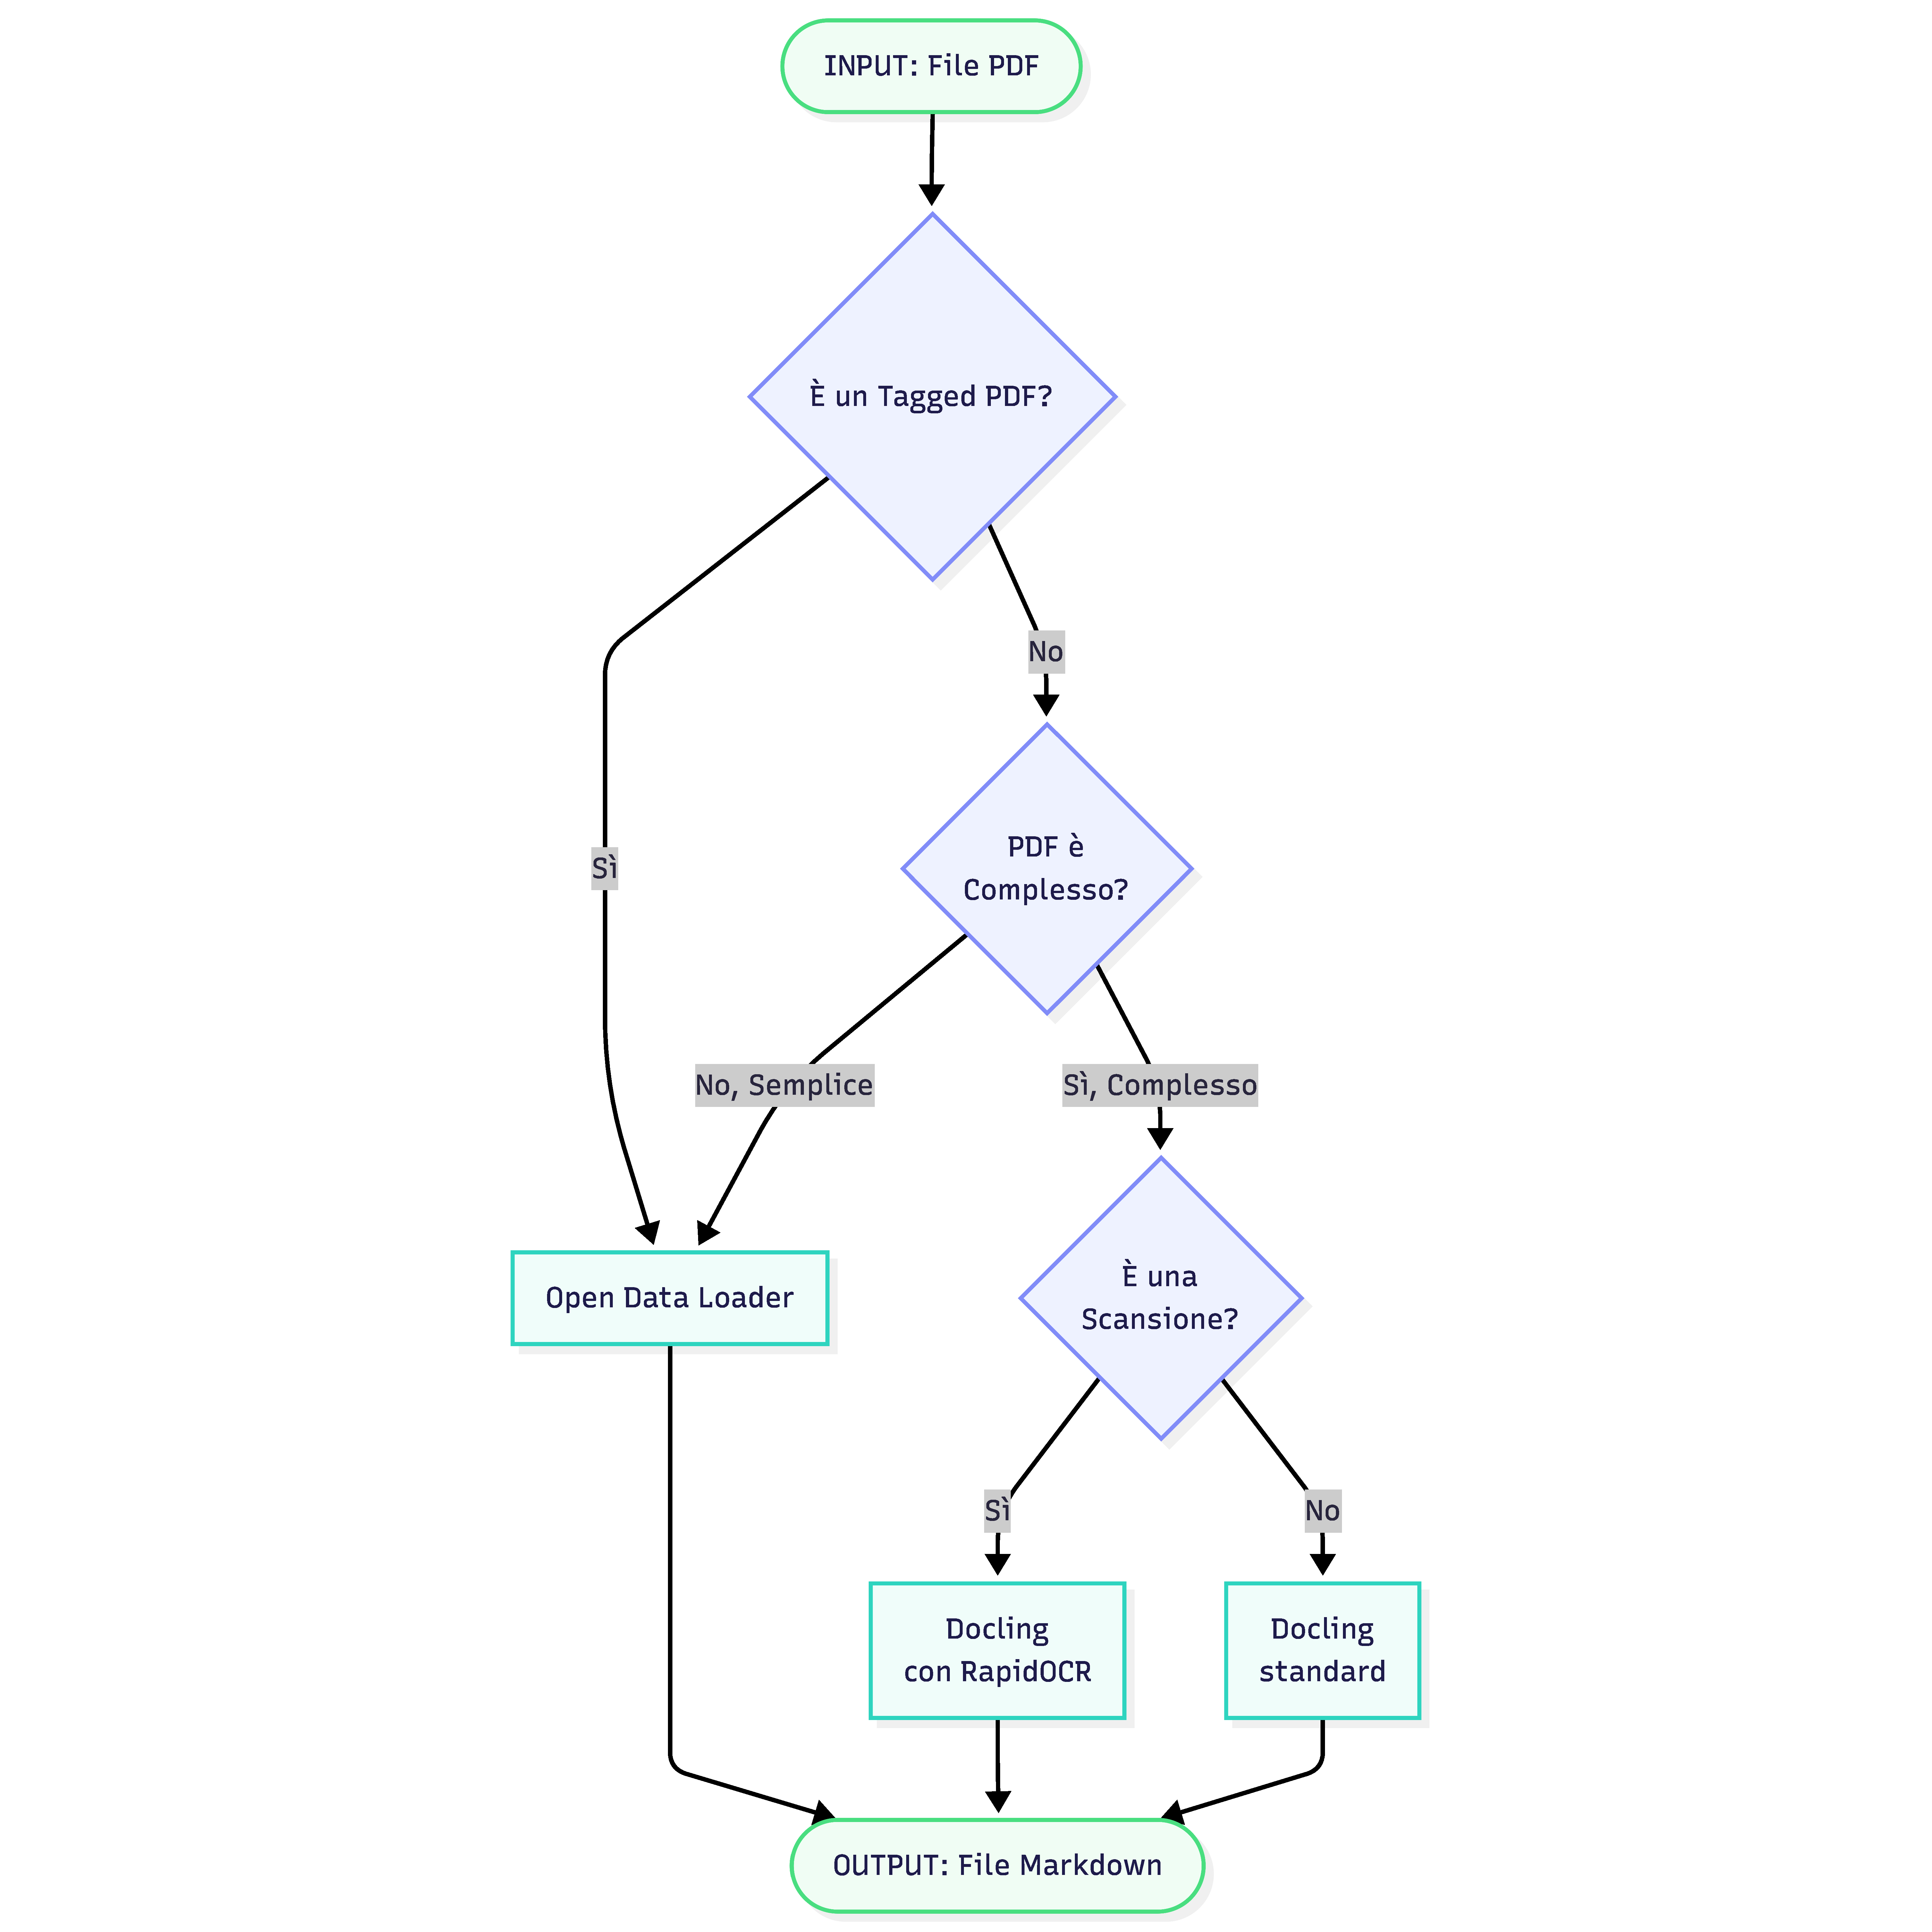
\includegraphics[width=1\textwidth]{_images/triage-processor.pdf}
    \caption{Flowchart del Custom Triage Processor}
    \label{fig:triage-processor}
\end{figure}
\newpage


\section{Strutturazione dei Documenti tramite LLM}
\label{sec:strutturazione_semantica}

Una volta ultimata la fase di estrazione del testo grezzo, illustrata nella sezione precedente, i documenti normativi si presentano sotto forma di file testuali piatti in formato Markdown. Tali file, pur contenendo l'intero testo originale, sono del tutto privi di metadati strutturali e di una formattazione gerarchica chiara. 
Poiché l'architettura di sistema prevede l'ingestione di questi documenti all'interno di un database a grafo (Neo4j) e in un database vettoriale (Qdrant), risulta indispensabile trasformare il testo non strutturato in una gerarchia rigorosa. L'archiviazione del solo testo grezzo, infatti, risulterebbe del tutto inadeguata e priva di utilità pratica. Una strutturazione accurata rappresenta il prerequisito fondamentale per abilitare qualsiasi operazione avanzata di \textit{information retrieval}, garantendo che i dati possano essere interrogati in modo efficiente e contestuale.

\subsection{Il Modello e la Strategia di Generazione}

Per affrontare il compito cruciale della strutturazione sintattica, è stato impiegato il Large Language Model \texttt{Gemini 3.5 Flash}. A livello di architettura software, il processo è diviso in due step distinti: la generazione di una struttura JSON gerarchica e l'estrazione delle relazioni semantiche tra le entità legali.

\subsection{Generazione della Struttura Gerarchica}

L'efficacia e l'accuratezza del processo di strutturazione si fondano su un \textit{System Prompt} ingegnerizzato ad hoc. Il suo compito principale è quello di mappare il contenuto all'interno del seguente schema logico:

\begin{itemize}
    \item \textbf{Metadati (\texttt{metadata}):} Il modello estrae e categorizza i dati identificativi dell'atto. Vengono isolati campi chiave come la data di stipula, il titolo completo e il nome del file originale.
    \item \textbf{Sezioni Introduttive e Conclusive:} Vengono separate dal corpo normativo tutte le sezioni di contorno. Tra queste figurano le premesse iniziali e le epigrafi (\texttt{preface}), gli indici (\texttt{preamble}), le dichiarazioni di chiusura con le relative firme (\texttt{conclusions}) e gli eventuali documenti annessi (\texttt{attachments}).
    \item \textbf{Corpo del Documento (\texttt{body}):} Rappresenta il nucleo dell'algoritmo di strutturazione. Il modello deve nidificare il testo seguendo fedelmente la gerarchia complessa e rigida tipica degli atti normativi italiani: \textbf{Titoli $>$ Capi $>$ Articoli $>$ Commi}.
\end{itemize}

Per garantire la massima coerenza dei dati all'interno del Knowledge Graph, sono state imposte al LLM regole tassative di parsing:

\begin{itemize}
    \item \textbf{Normalizzazione Numerica:} Tutti gli identificativi gerarchici originariamente espressi in numeri romani o in forma testuale (es. ``TITOLO I'', ``CAPO IV'') devono essere categoricamente convertiti in numeri interi arabi (1, 4, ecc.).
    \item \textbf{Gestione Dinamica dei Commi:} Poiché nei testi di legge i commi non sono sempre esplicitamente numerati, il modello è istruito a dedurli analizzando le interruzioni logiche dei paragrafi, assegnando loro una numerazione progressiva.
    \item \textbf{Ottimizzazione dello Schema:} Per mantenere leggeri i file JSON, il modello è programmato per non inizializzare chiavi con valori vuoti o nulli; se un livello gerarchico (come un Capo o un Titolo) non trova riscontro nel testo originale, la proprietà viene semplicemente omessa.
\end{itemize}

L'esecuzione di questo processo restituisce una directory di documenti JSON puliti e strutturati gerarchicamente, pronti per essere archiviati e per affrontare il successivo step: l'estrazione delle relazioni semantiche tra le entità legali.

\subsection{Estrazione delle Relazioni Semantiche}

La sola scomposizione del testo normativo in una struttura gerarchica ad albero rappresenta una condizione necessaria ma non sufficiente per la costruzione di un vero e proprio \textit{Knowledge Graph}. Per sfruttare appieno la potenza topologica di un database a grafo come Neo4j, è indispensabile individuare e mappare esplicitamente i collegamenti e le dipendenze logiche che intercorrono tra le diverse disposizioni giuridiche all'interno dello stesso atto. A questo scopo, la pipeline prevede un secondo step logico interamente dedicato all'estrazione delle relazioni semantiche.
In questa fase, l'input non è più il testo grezzo, ma i file JSON prodotti nello step precedente, che quindi agiscono come una base di conoscenza consolidata. Ciascun documento viene quindi analizzato dal LLM \texttt{Gemini 3.5 Flash}, guidato da un \textit{System Prompt} specializzato. Tale prompt è stato progettato per riconoscere i costrutti linguistici del gergo giuridico che indicano un collegamento formale tra le parti del testo. Le relazioni estratte sono:
\begin{itemize}
    \item \textbf{CITA:} Un articolo o comma fa riferimento a un'altra disposizione.
    \item \textbf{ABROGA:} Una disposizione annulla la validità giuridica di un'altra.
    \item \textbf{DEROGA:} Un elemento introduce un'eccezione a una regola generale.
    \item \textbf{SOSTITUISCE:} Una disposizione prende il posto di un'altra.
    \item \textbf{INTERPRETA:} La comprensione di una norma dipende dalla lettura di un'altra.
\end{itemize}

L'output di questa analisi è una rete di collegamenti formali, dove per ciascuna relazione vengono specificati il nodo di partenza, il nodo di arrivo e il tipo di legame. Queste informazioni sono esportate in un nuovo set di file JSON.

Questo approccio a due stadi permette di separare le responsabilità e ridurre il carico cognitivo del modello a ogni ciclo. In questo modo si produce un dataset pulito e affidabile, pronto per essere caricato nel grafo.

\section{Importazione dati nei Database}
\label{sec:database_ingestion}

Una volta completata la strutturazione dei documenti legali in formato JSON, si apre la fase di persistenza e indicizzazione dei dati. Nel contesto di questo progetto di tirocinio, l'architettura prevede il caricamento dei dati estratti all'interno del database a grafo Neo4j.

Per garantire la flessibilità e favorire un ambiente di sviluppo pulito e modulare, lo sviluppo del software ha visto l'applicazione del \textit{Repository Pattern} e l'uso di interfacce polimorfiche.

\subsection{I Modelli di Dominio}
\label{sec:modelli_dominio}
Prima di analizzare le strategie di persistenza, è fondamentale descrivere come i dati estratti vengano rappresentati. All'interno della cartella \texttt{models} di questo step, il sistema definisce le entità fondamentali del dominio normativo utilizzando il paradigma ad oggetti. Queste classi operano essenzialmente come \textit{Entities}: strutture dati pure, prive di logica di persistenza diretta o dipendenze verso i DBMS, il cui unico scopo è incapsulare i dati del dominio.

L'architettura dei modelli è rappresentata nel diagramma UML della Figura \ref{fig:domain-models-class-diagram}. Le principali classi sono:
\begin{itemize}
    \item \texttt{Entity}: Incapsula l'ente pubblico emittente, memorizzando i metadati di dominio.
    \item \texttt{LegalAct}: È la classe orchestratrice principale. Rappresenta l'atto legale nella sua interezza e contiene i metadati principali (title, publication\_date, file\_name) e soprattutto una lista \texttt{elements} che tiene traccia di tutti i sotto-elementi istanziati e delle loro relazioni gerarchiche.
    \item \texttt{StructuralElement}: È la classe base polimorfica per mappare le sottoclassi \texttt{Title}, \texttt{Chapter} e \texttt{Article}, mantenendo traccia del numero d'ordine e dell'eventuale rubrica.
    \item \texttt{Paragraph}: Rappresenta il comma ed è l'unità atomica d'informazione sulla quale verranno calcolati gli embedding.
\end{itemize}

\begin{figure}[H]
    \centering
    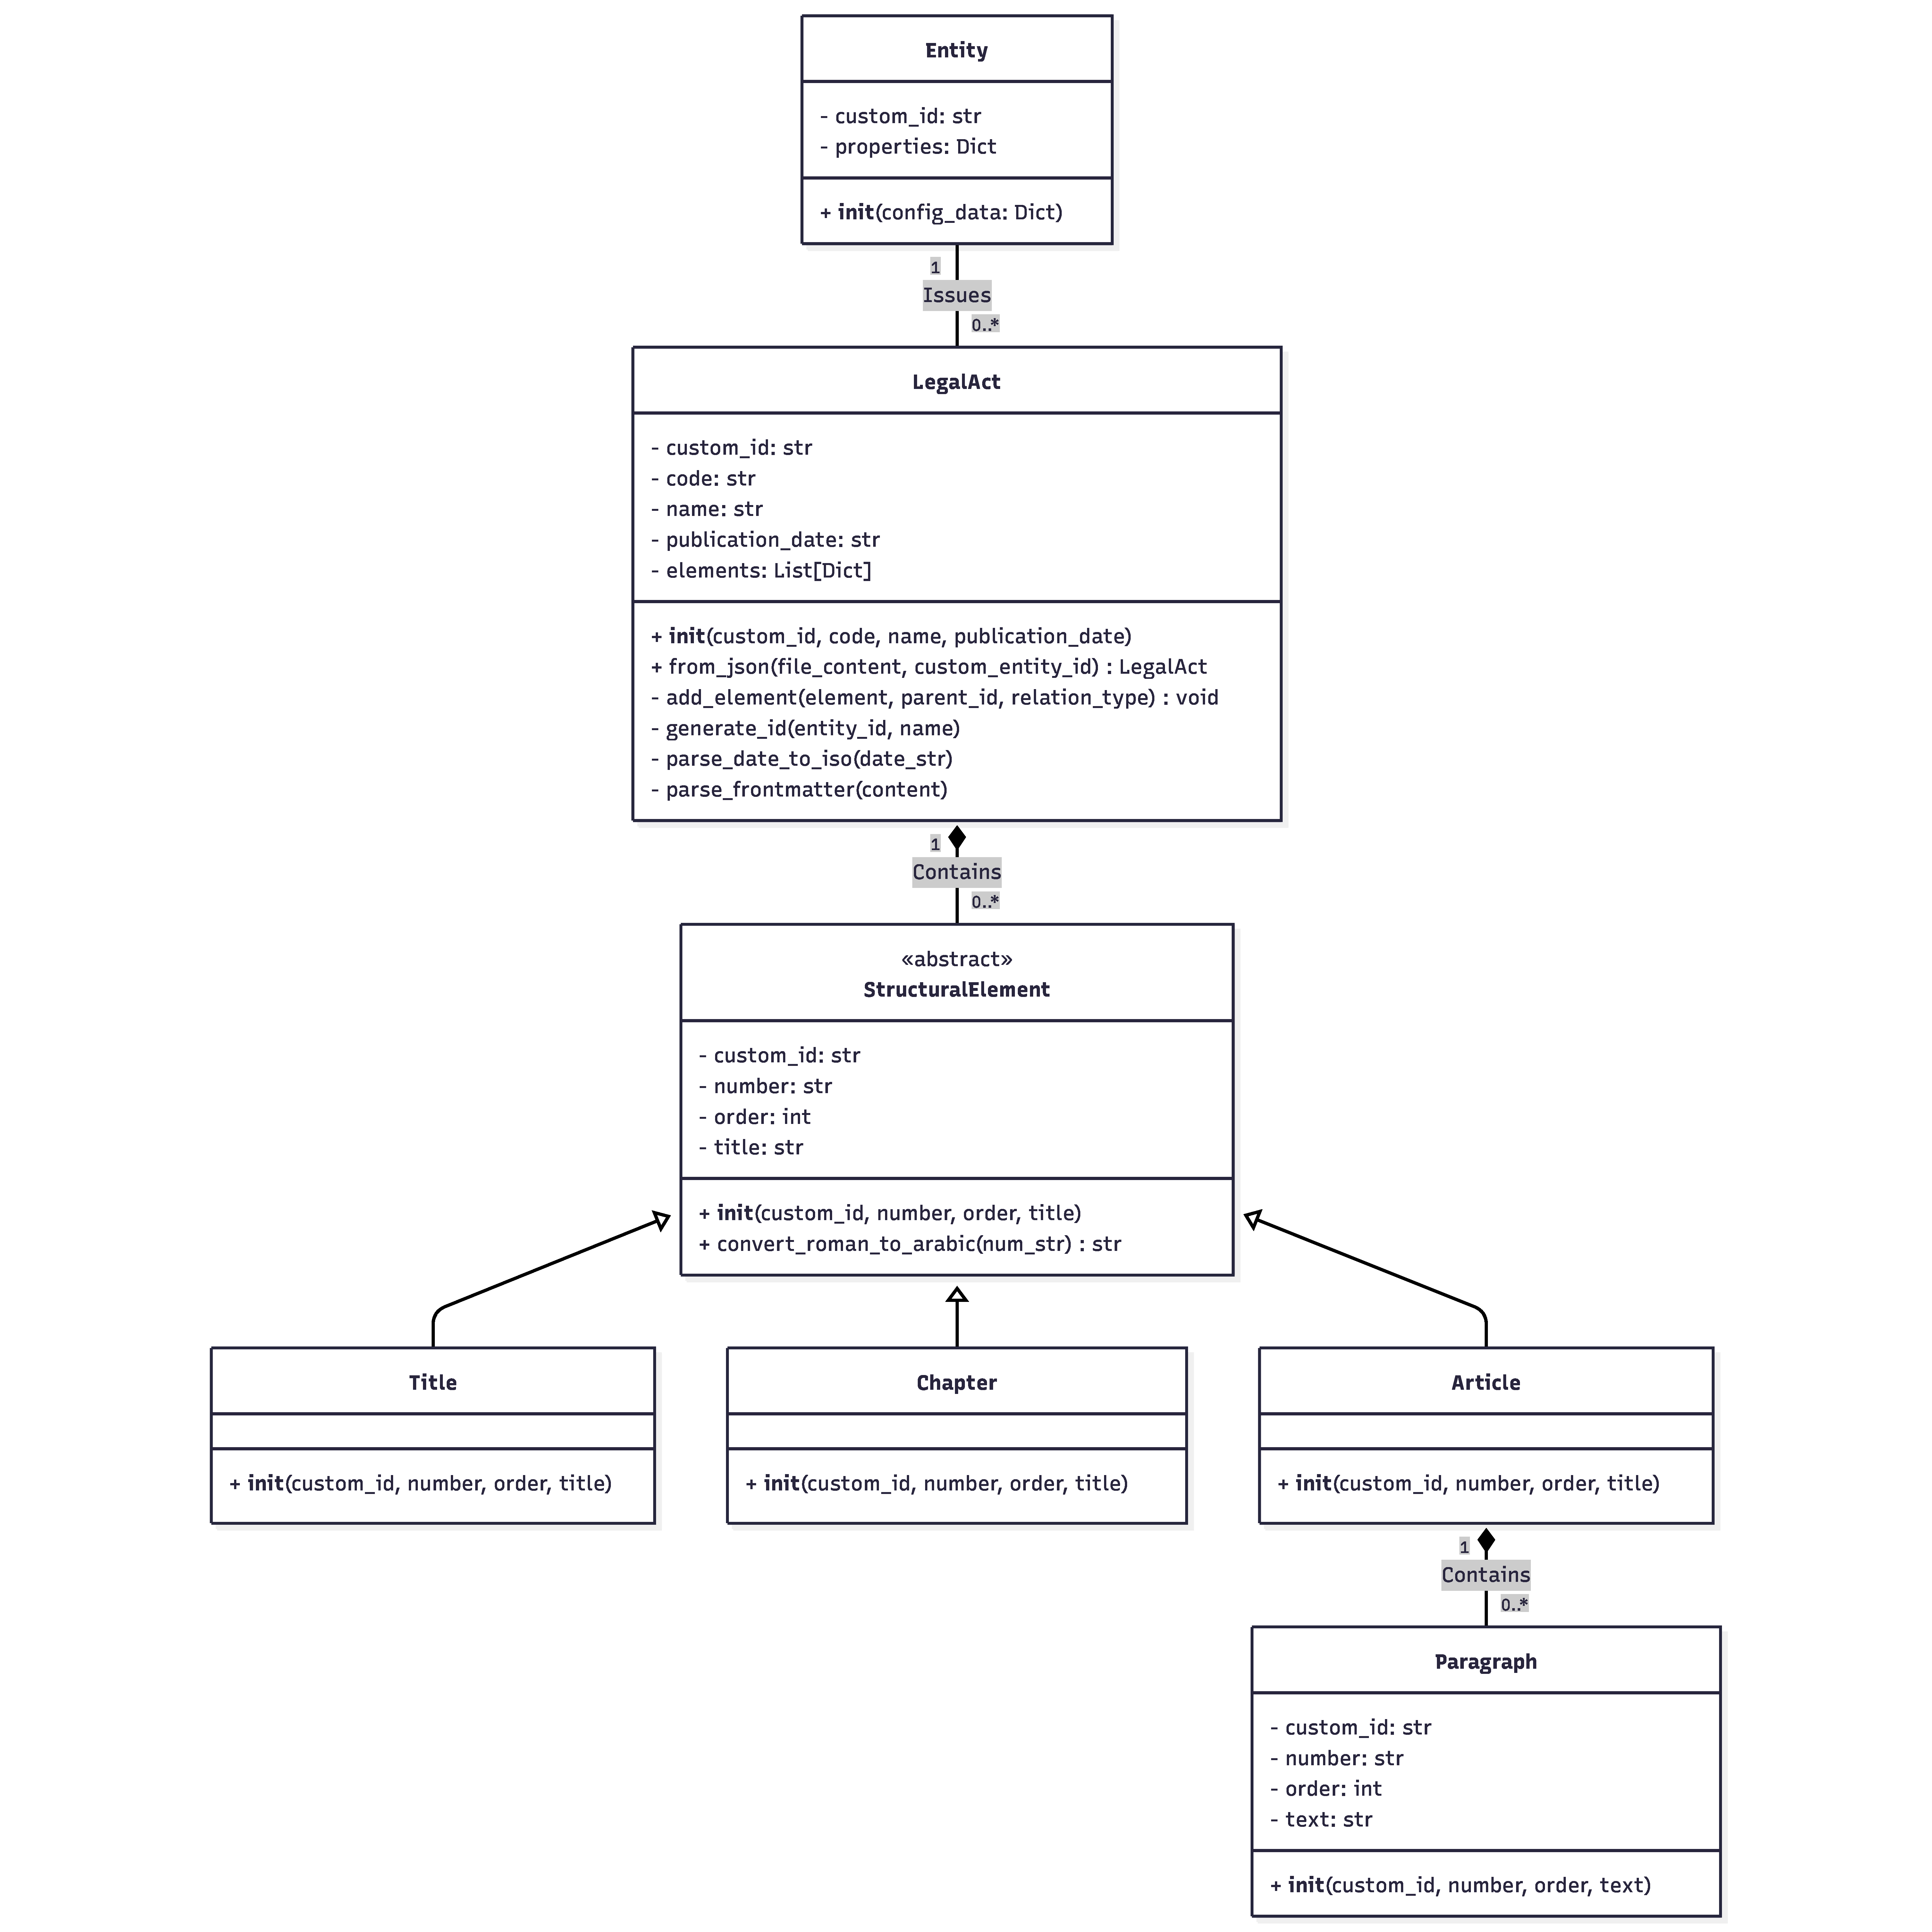
\includegraphics[width=1\textwidth]{_images/domain-models-class-diagram.pdf}
    \caption{Class Diagram dei modelli di dominio}
    \label{fig:domain-models-class-diagram}
\end{figure}


\subsection{Interfaccia per il disaccoppiamento della persistenza}
L'adozione di un'interfaccia comune di importazione nasce dalla precisa volontà di disaccoppiare la logica di lettura dei dati dalla loro effettiva persistenza fisica.
Sebbene l'attuale implementazione preveda l'utilizzo esclusivo del database a grafo Neo4j, questa scelta architetturale si rivela strategica per sviluppi futuri. Qualora si rendesse necessario integrare nuovi DBMS (ad esempio, un database puramente vettoriale dedicato esclusivamente agli embedding), sarà sufficiente implementare una nuova classe concreta senza dover alterare il flusso principale del programma. Inoltre, il disaccoppiamento garantisce un'elevata testabilità del codice, permettendo di validare la logica di dominio e il parsing dei documenti simulando le operazioni di salvataggio indipendentemente dal database sottostante.

Nel sistema sviluppato, l'interfaccia astratta di riferimento è rappresentata dalla classe \texttt{DBImporterInterface}. Essa definisce tre metodi fondamentali che ogni classe concreta deve implementare:
\begin{itemize}
    \item \texttt{connect()}: per la gestione e la validazione della connessione con l'istanza specifica del database;
    \item \texttt{import\_legal\_act(entity, legal\_act)}: per l'esecuzione effettiva di ingestion dell'atto normativo e dell'ente emittente;
    \item \texttt{close()}: per la chiusura sicura delle sessioni.
\end{itemize}


\subsection{Architettura del Database Neo4j}
\label{subsec:neo4j_architecture}

Il database modella fedelmente l'albero gerarchico discendente del documento, garantendo la flessibilità necessaria per gestire percorsi diretti qualora i livelli intermedi siano stati omessi durante la strutturazione JSON (es. \texttt{LegalAct $\rightarrow$ Article $\rightarrow$ Paragraph}). 

Le \textit{Label} dei nodi sul grafo (ovvero \textbf{Entity}, \textbf{LegalAct}, \textbf{Title}, \textbf{Chapter}, \textbf{Article} e \textbf{Paragraph}) riflettono rigorosamente la struttura delle classi di dominio già presentate nella Sezione \ref{sec:modelli_dominio}, così proprio come le \textit{Properties} dei nodi, che conservano i metadati principali e le informazioni testuali.

Un aspetto architetturale chiave, comune a tutti i nodi, è la presenza della proprietà \texttt{custom\_id}. Tale attributo codifica per intero il percorso gerarchico del nodo all'interno del documento (ad esempio, \texttt{ente\_\_atto\_\_title-1\_\_chapter-2\_\_article-3\_\_paragraph-4}). Grazie a questo approccio, il database può sfruttare l'indicizzazione su questa proprietà per individuare immediatamente un singolo nodo, azzerando le operazioni di attraversamento del grafo e garantendo un recupero delle informazioni in tempo costante.

All'interno di questa topologia, i nodi di tipo \textbf{Paragraph} ricoprono un ruolo centrale per le funzionalità avanzate del sistema. Oltre a conservare le proprietà testuali, in questi nodi vengono salvate le rappresentazioni vettoriali dei dati: in particolare, gli embedding semantici a dimensione variabile e un embedding strutturale a 128 dimensioni calcolato mediante l'algoritmo di \textit{Node2Vec} (maggiori informazioni sono nel capitolo \ref{sec:creazione_embedding}). L'archiviazione di tali vettori è progettata per abilitare le successive operazioni di interrogazione.

L'ecosistema di relazioni (\textit{Edges}) all'interno del grafo si articola in tre macro-categorie progettate per supportare le interrogazioni avanzate:
\begin{itemize}
    \item \textbf{Relazioni Strutturali}: Definiscono la topologia discendente del documento normativo. Comprendono l'arco \texttt{ISSUES} che lega l'Ente all'Atto, e la catena di contenimento gerarchico formata da \texttt{HAS\_TITLE}, \texttt{HAS\_CHAPTER}, \texttt{HAS\_ARTICLE} e \texttt{HAS\_PARAGRAPH}.
    \item \textbf{Relazioni Sequenziali}: I commi appartenenti allo stesso articolo sono concatenati linearmente tramite la relazione \texttt{NEXT\_PARAGRAPH}. Questa architettura a lista concatenata si rivela fondamentale per espandere dinamicamente la finestra di contesto durante la fase di interrogazione, permettendo di recuperare i commi logicamente antecedenti o successivi senza dover eseguire query computazionalmente costose per ricalcolare l'ordine strutturale.
    \item \textbf{Relazioni Legali}: Traducono in archi orientati sul grafo i collegamenti logici e giuridici intra-documento individuati dal prompt specializzato dell'LLM (Sezione \ref{sec:strutturazione_semantica}). Le cinque tipologie di relazione estratte vengono trasposte fedelmente nelle label \texttt{CITES}, \texttt{REPEALS}, \texttt{INTERPRETS}, \texttt{REPLACES} e \texttt{DEROGATES}. 
\end{itemize}

Occorre precisare che, sebbene lo schema dati supporti nativamente tutte le interazioni legali sopracitate, l'attuale popolamento del database non registra occorrenze per le relazioni \texttt{REPEALS} e \texttt{REPLACES}. Questa mancanza non è imputabile a un difetto del sistema di estrazione, bensì rappresenta un limite intrinseco dei documenti elaborati, che non contengono clausole esplicite di abrogazione o sostituzione strutturata.

\subsection{Dettagli Implementativi dell'Ingestion su Neo4j}
Un atto legale non può essere salvato tramite un'unica operazione atomica standard, a causa delle complesse connessioni tra i nodi, per questo motivo la responsabilità è stata distribuita su una serie di repository specializzati, ognuno deputato alla gestione del ciclo di vita di un singolo modello di dominio:
\begin{itemize}
    \item \texttt{EntityRepository}: Gestisce l'inserimento dei nodi relativi agli enti istituzionali.
    \item \texttt{LegalActRepository}: Inserisce il nodo radice dell'atto e lo ancora all'ente emittente.
    \item \texttt{StructuralElementRepository}: Incapsula la logica Cypher necessaria a creare i nodi intermedi del grafo e gli archi verso i rispettivi nodi padri.
    \item \texttt{ParagraphRepository}: Si occupa esclusivamente della persistenza dei nodi foglia contenenti il testo dei commi.
\end{itemize}

Per quanto riguarda il salvataggio delle relazioni trasversali, queste informazioni vengono lette da file JSON esterni dedicati (Sezione \ref{sec:estrazione_relazioni}), per poi essere elaborate da un metodo che, attraverso i \texttt{custom\_id} dei nodi salvati e indicizzati sul grafo, trova in maniera quasi istantanea i nodi correlati dall'estratto JSON ed esegue una query Cypher dedicata per la creazione dell'arco semantico.

\begin{lstlisting}[language=Cypher, caption={Query Cypher per l'inserimento delle relazioni legali}, label={lst:cypher_relationships}]
MATCH (s {custom_id: $source_id})
WITH s
MATCH (t {custom_id: $target_id})
MERGE (s)-[r:`<rel_type>`]->(t)
RETURN r
\end{lstlisting}

\noindent L'obiettivo di questa query è rintracciare i due nodi di interesse (sorgente e destinazione) tramite il loro identificativo univoco e stabilire una relazione orientata tra di essi.

Di seguito troviamo un esempio di relazione estratta in formato JSON, con ID parzialmente omessi per motivi di leggibilità:

\begin{lstlisting}[caption={Esempio reale di relazione estratta in formato JSON}, label={lst:json-cites}, breaklines=true]
{
  "sourceId": "ente-provincia-taranto__contratto-collettivo-[...]__title-2__chapter-2__article-8__paragraph-6",
  "relationshipType": "CITES",
  "targetId": "ente-provincia-taranto__contratto-collettivo-[...]__title-2__chapter-2__article-8__paragraph-1"
}
\end{lstlisting}

A supporto di quanto descritto, la Figura \ref{fig:relationship_example} fornisce una rappresentazione visiva delle relazioni instaurate tra i nodi dell'articolo 8 del seguente atto: \texttt{"CCNL del personale non dirigente del comparto regioni e autonomie locali"}

\begin{figure}[H]
    \centering
    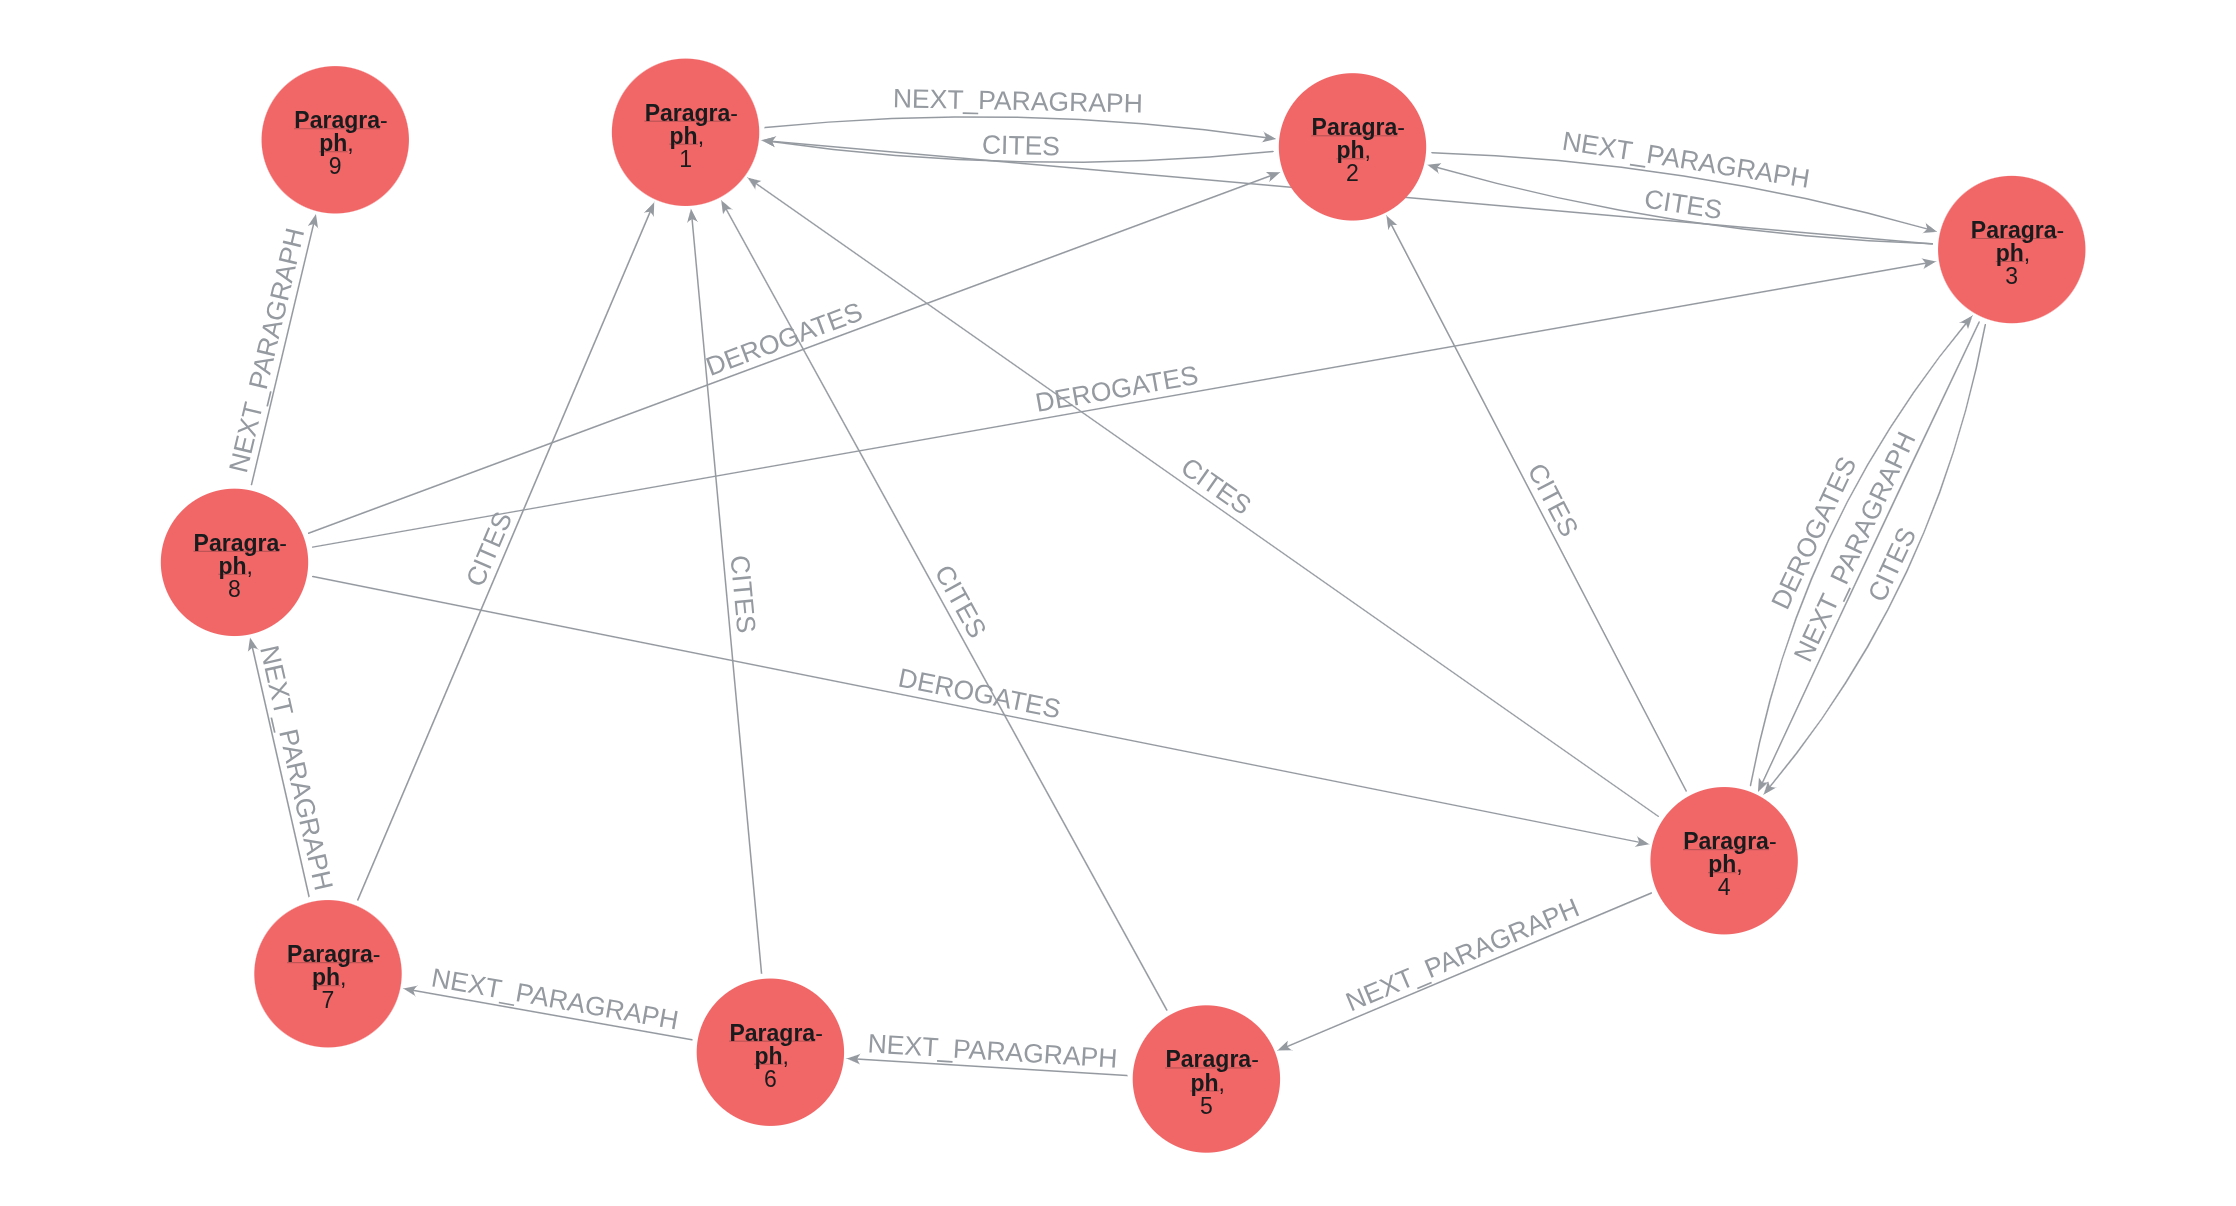
\includegraphics[width=1\textwidth]{_images/relationship.png}
    \caption{Rappresentazione visiva delle relazioni instaurate tra i nodi dell'articolo 8 di un atto normativo.}    
    \label{fig:relationship_example}
\end{figure}

\subsection{Risultati e Metriche}
L'esecuzione della pipeline di ingestion ha dimostrato un'elevata efficienza, completando il caricamento dell'intero dataset all'interno del database in un tempo complessivo di \textbf{50.29 secondi}.

Il processo ha popolato il grafo con un totale di 8.535 nodi e 14.201 relazioni. Di seguito viene riportato il dettaglio quantitativo delle entità di dominio e degli archi salvati.

La Tabella \ref{tab:statistiche_nodi} illustra la distribuzione dei nodi all'interno del grafo, raggruppati per \textit{Label}. Come si può osservare dai dati, vi è una netta preponderanza numerica dei nodi \texttt{Paragraph}, i quali rappresentano l'unità atomica d'informazione su cui si basano le successive operazioni di embedding e ricerca.

\begin{table}[H]
    \centering
    \renewcommand{\arraystretch}{1.2}
    \begin{tabular}{|l|r|}
        \hline
        \textbf{Label Nodo} & \textbf{Quantità} \\
        \hline
        \texttt{Paragraph} & 6.396 \\
        \texttt{Article} & 1.802 \\
        \texttt{Chapter} & 147 \\
        \texttt{LegalAct} & 95 \\
        \texttt{Title} & 93 \\
        \texttt{Entity} & 2 \\
        \hline
    \end{tabular}
    \caption{Statistica dei nodi inseriti nel database Neo4j.}
    \label{tab:statistiche_nodi}
\end{table}

Per quanto riguarda invece le interconnessioni tra le entità, la Tabella \ref{tab:statistiche_relazioni} dettaglia il conteggio esatto degli archi strutturali, sequenziali e legali creati durante l'importazione.

\begin{table}[H]
    \centering
    \renewcommand{\arraystretch}{1.2}
    \begin{tabular}{|l|r|}
        \hline
        \textbf{Tipo di Relazione} & \textbf{Quantità} \\
        \hline
        \texttt{HAS\_PARAGRAPH} & 6.396 \\
        \texttt{NEXT\_PARAGRAPH} & 4.594 \\
        \texttt{HAS\_ARTICLE} & 1.802 \\
        \texttt{CITES} & 1.030 \\
        \texttt{HAS\_CHAPTER} & 147 \\
        \texttt{ISSUES} & 95 \\
        \texttt{HAS\_TITLE} & 93 \\
        \texttt{DEROGATES} & 41 \\
        \texttt{INTERPRETS} & 3 \\
        \hline
    \end{tabular}
    \caption{Statistica delle relazioni inserite nel database Neo4j.}
    \label{tab:statistiche_relazioni}
\end{table}

Come si evince dalla Tabella \ref{tab:statistiche_relazioni}, l'analisi degli archi conferma la solidità dell'architettura a lista concatenata, evidenziata dal notevole volume di relazioni \texttt{NEXT\_PARAGRAPH} (4.594), essenziali per l'espansione dinamica del contesto in fase di retrieval. 

Inoltre, analizzando sempre i medesimi dati in merito agli archi logico-legali, si osserva una netta predominanza delle relazioni di citazione (\texttt{CITES}, 1.030 occorrenze), seguite da un numero minoritario di deroghe (\texttt{DEROGATES}, 41) e interpretazioni (\texttt{INTERPRETS}, 3). Coerentemente con quanto anticipato nella Sezione \ref{subsec:neo4j_architecture}, le metriche riportate confermano l'assenza totale di occorrenze per le relazioni di abrogazione (\texttt{REPEALS}) e sostituzione (\texttt{REPLACES}) all'interno di questo specifico bacino documentale.

\subsection{Visualizzazione del Grafo}
A conclusione di questo capitolo, si propone una rappresentazione visiva di un estratto del database Neo4j volta a mostrare in maniera intuitiva la topologia della rete. Nella Figura \ref{fig:graph-visualization} è possibile osservare la struttura gerarchica e le connessioni tra le diverse entità, evidenziate mediante una differenziazione cromatica:
\begin{itemize}
    \item I \textbf{nodi gialli} rappresentano l'ente emittente (\texttt{Entity});
    \item I \textbf{nodi azzurri} indicano gli atti legali (\texttt{LegalAct});
    \item I \textbf{nodi rossi} corrispondono ai commi (\texttt{Paragraph});
    \item I \textbf{restanti nodi} raffigurano le altre parti della gerarchia strutturale del documento, ossia i titoli (\texttt{Title}), i capi (\texttt{Chapter}) e gli articoli (\texttt{Article}).
\end{itemize}

\begin{figure}[H]
    \centering
    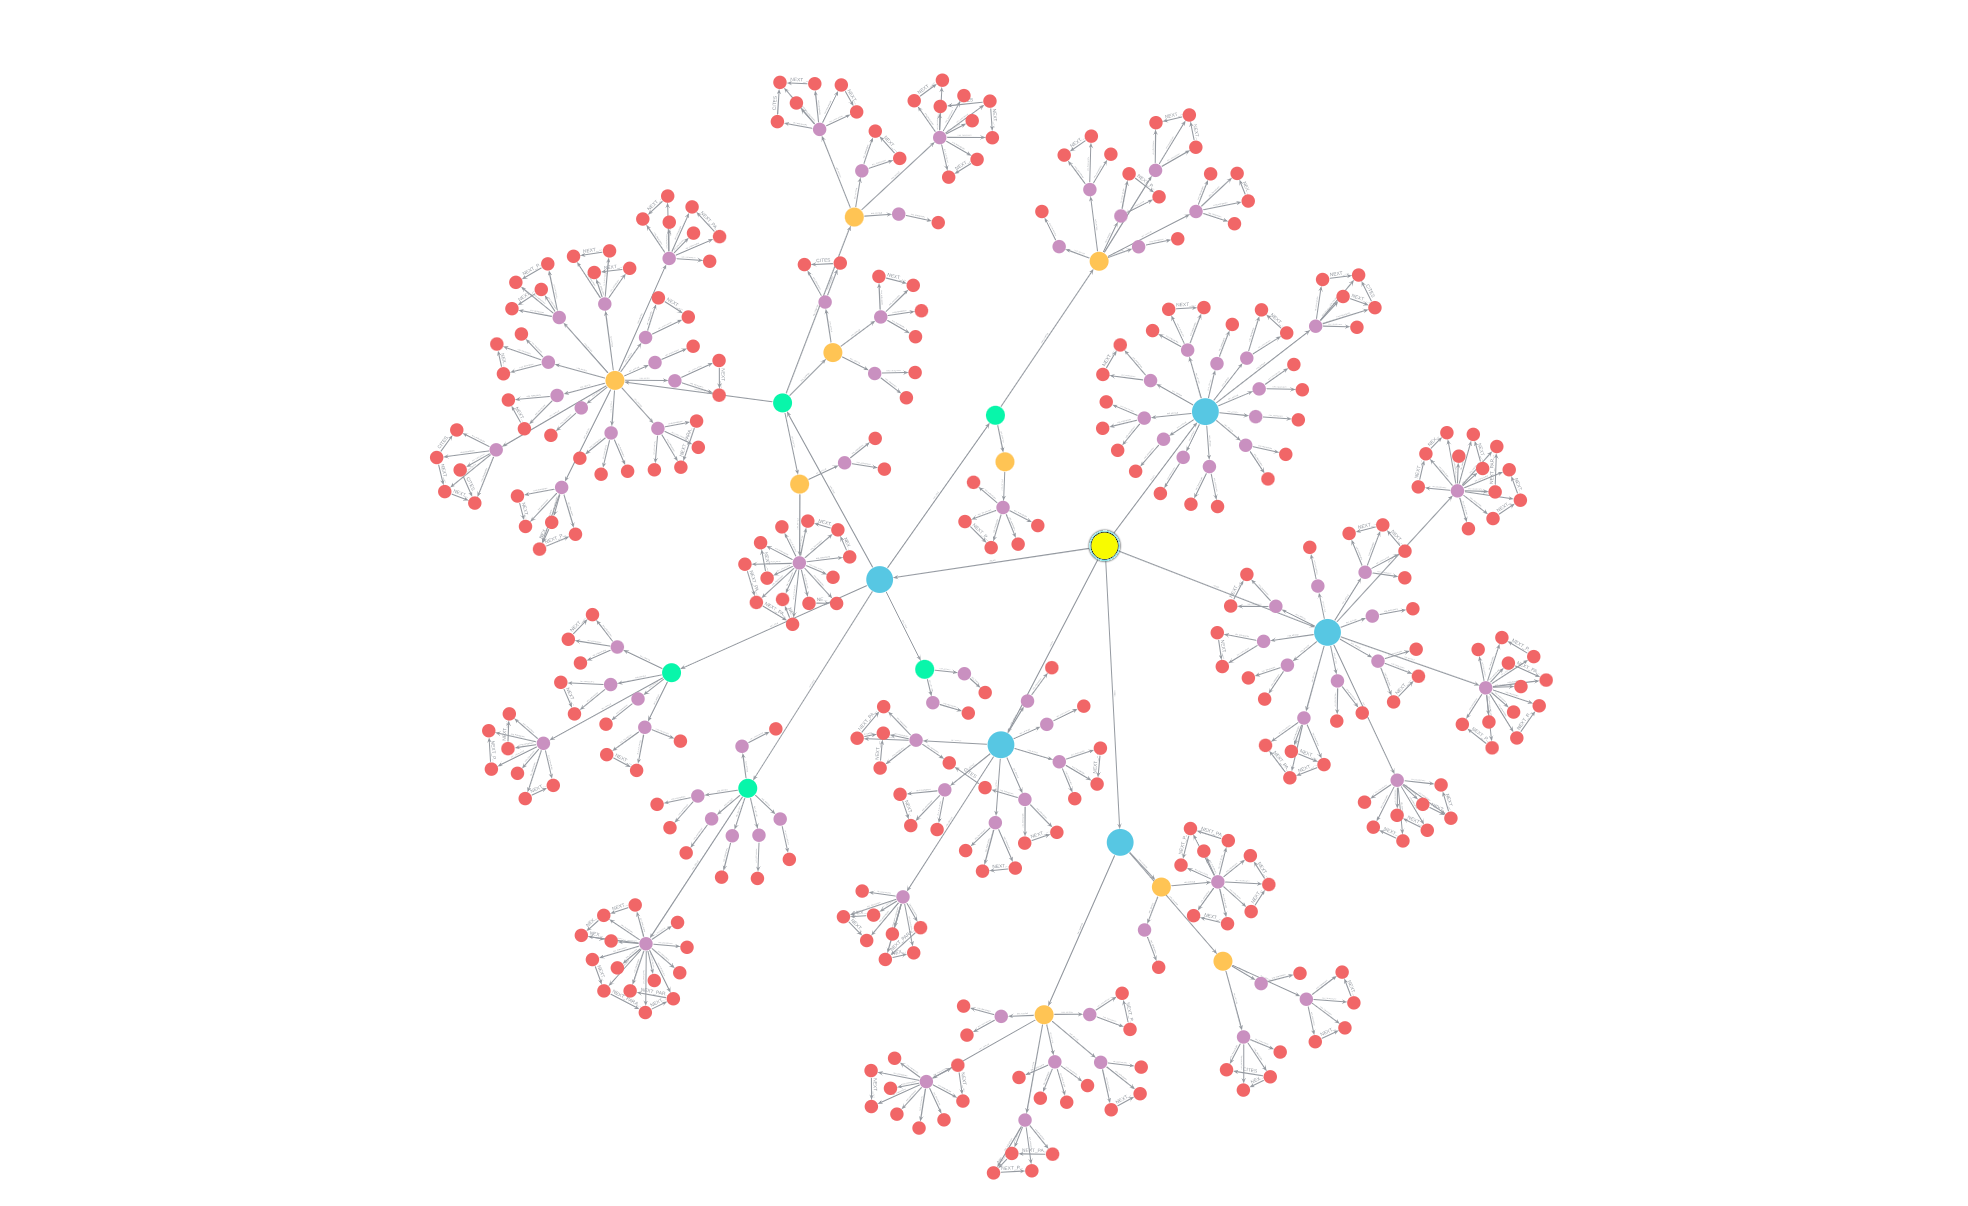
\includegraphics[width=1\textwidth]{_images/graph-visualization.png}
    \caption{Rappresentazione visiva di un estratto del database a grafo Neo4j.}
    \label{fig:graph-visualization}
\end{figure}

\newpage
\section{Creazione degli Embedding}
\label{sec:creazione_embedding}

L'operazione di vettorizzazione, o di \textit{embedding}, rappresenta un passaggio cruciale per abilitare le funzionalità di ricerca semantica all'interno del database a grafo.
La pipeline supporta tre modelli di embedding, dettagliati nella sezione \ref{sec:llm_embedding_models}: 
\begin{itemize}
    \item \texttt{google/embeddinggemma-300m}
    \item \texttt{perplexity-ai/pplx-embed-v1-0.6b}
    \item \texttt{perplexity-ai/pplx-embed-context-v1-0.6b}
\end{itemize}

I vettori vengono archiviati direttamente come proprietà all'interno dei nodi (\texttt{:Paragraph}) già esistenti nel grafo. Questo evita la necessità di un database vettoriale separato e consente al modello di ricerca di operare direttamente su Neo4j.

Neo4j, inoltre, supporta la creazione di indici vettoriali utilizzando algoritmi di ricerca approssimata (\textit{Approximate Nearest Neighbor Search}, ANN). Invece di calcolare la distanza coseno tra il vettore di query e tutti gli altri vettori (operazione $O(n)$ molto costosa), questi indici riducono drasticamente lo spazio di ricerca. Di conseguenza, il tempo di esecuzione delle query passa da secondi a millisecondi, rendendo la ricerca praticabile anche su documenti normativi di grandi volumi.

\subsection{Differenza nell'Arricchimento Contestuale: Standard vs Late Chunking}
\label{subsec:arricchimento_contestuale}
 
Il sistema implementa due approcci diversi per fornire \textit{contesto} ai commi. Se si fornisce al modello solo la stringa del comma \textquote{... è punito con la reclusione da 1 a 3 anni}, l'embedding generato risulterà limitato, poiché il testo manca di informazioni fondamentali come il soggetto e il reato specifico (elementi definiti nei livelli superiori come l'articolo o il titolo).
Ecco come le due metodologie risolvono il problema:
 
\subsubsection{A. Arricchimento Standard (Modelli: Gemma 300m e PPLX-v1)}
 
In questo approccio, il contesto viene iniettato testualmente attraverso \textit{String Concatenation}.
Per ciascun comma, viene recuperato il contesto gerarchico risalendo l'albero strutturale tramite query Cypher. Tutte queste informazioni vengono concatenate in un'unica stringa, producendo un testo inviato al modello simile al seguente:

\begin{center}
    \texttt{\textquote{Atto: Codice Penale | Titolo 3 Dei delitti contro l'amministrazione della giustizia | Capo 2 Dei delitti contro l'autorità delle decisioni giudiziarie | Art. 385 Evasione | Comma 1 | ... è punito con la reclusione da 1 a 3 anni.}}
\end{center}

In questo approccio, ogni comma viene trattato come un \textit{chunk isolato} al momento dell'embedding. Sebbene il modello riceva il testo arricchito dai metadati gerarchici, il contesto rimane limitato a questo preambolo testuale statico.
 
\subsubsection{B. Arricchimento tramite Late Chunking (Modello: PPLX-Context)}
 
Questo approccio impiega una vera e propria contestualizzazione a livello di rete neurale. A differenza dell'approccio standard, non utilizza preamboli testuali pre-calcolati, ma affida la comprensione semantica direttamente all'algoritmo di \textit{self-attention} del modello.

Il sistema recupera dal database, tramite query Cypher, l'intero articolo con tutti i commi che lo compongono, mantenendo traccia dell'ordine sequenziale e dei confini esatti tra di essi. Invece di frammentare il testo a monte e inviare al modello i commi singolarmente, il sistema li presenta all'encoder come un'unica sequenza di input ininterrotta.

È in questa fase che agisce il meccanismo di \textit{late chunking}. Il modello processa l'articolo nella sua interezza attraverso i successivi layer del Transformer; in questo modo, la \textit{self-attention} bidirezionale permette ai token di ciascun comma di "prestare attenzione" e interagire con i token adiacenti e con l'intero testo. Questo approccio abbatte i confini artificiali del chunking testuale, permettendo alla rete di risolvere dinamicamente pronomi, riferimenti incrociati e concetti impliciti basandosi sul contesto normativo globale.

Solo nella fase finale, dopo che ogni singolo token ha assorbito un significato profondamente contestualizzato, il modello applica un'operazione di \textit{pooling} differenziata. Sfruttando gli indici sequenziali salvati in precedenza, estrae e restituisce gli embeddings separati per ciascun comma originale. Questa architettura garantisce che l'embedding finale di un singolo comma racchiuda non solo il suo significato letterale, ma anche le sfumature semantiche derivanti dal resto dell'articolo, unendo la massima precisione granulare a una perfetta consapevolezza del contesto globale.

Un esempio pratico:

\begin{quote}
\texttt{Comma 1: "I soggetti che omettono la dichiarazione dei redditi sono puniti con una sanzione di 1.000 euro."}

\texttt{Comma 2: "La disposizione non si applica se essi dimostrano l'assenza di dolo."}
\end{quote}

Se il modello processa il Comma 2 in isolamento, la parola "essi" è ambigua e "La disposizione" è un concetto vuoto.
Sfruttando il late chunking, la rete neurale collega istantaneamente "essi" del Comma 2 ai "soggetti" del Comma 1, e "La disposizione" all'intero concetto di sanzione appena letto.

\subsection{Il Graph Embedding come appoggio agli Embedding Semantici}
Oltre all'analisi puramente testuale, il sistema arricchisce la rappresentazione della conoscenza integrando l'informazione strutturale del documento. A tale scopo viene impiegato l'algoritmo \textbf{Node2Vec}, eseguito tramite la libreria Graph Data Science (GDS). Questo approccio genera un \textit{graph embedding} per ogni comma, codificando in vettori a 128 dimensioni la topologia della rete, ovvero la gerarchia del documento e le relazioni logico-giuridiche che legano i nodi. In questo modo, l'algoritmo mappa in regioni vicine dello spazio vettoriale quei commi che, a prescindere dal testo, condividono una medesima posizione strutturale o forti vincoli normativi.
Per adattare Node2Vec al dominio legale, la strategia di esplorazione del grafo tramite \textit{random walk} è stata calibrata attraverso i parametri \textbf{p} e \textbf{q}:
\begin{itemize}
    \item \textbf{Return parameter ($p = 1$)}: Mantiene un comportamento esplorativo neutrale, senza forzare né penalizzare il ritorno immediato al nodo precedente.
    \item \textbf{In-out parameter ($q = 0.5$)}: Essendo inferiore a $1$, forza un'esplorazione profonda (simile a una \textit{Depth-First Search}). Questa scelta è essenziale nel dominio legale, in quanto permette all'algoritmo di attraversare in profondità l'intera struttura verticale del documento (Legge $\rightarrow$ Titolo $\rightarrow$ Capo $\rightarrow$ Articolo $\rightarrow$ Comma) e di seguire agevolmente lunghe catene di rimandi normativi.
\end{itemize}
Inoltre, per guidare attivamente l'apprendimento verso i percorsi più significativi, è stato implementato un sistema di pesi differenziati per le diverse tipologie di relazione. Questi valori alterano le probabilità di transizione durante le passeggiate aleatorie, forzando il modello a privilegiare specifiche tipologie di relazioni:
\begin{itemize}
    \item \textbf{Pesi Elevati (2.0)}: Assegnati alle relazioni strutturali (\texttt{HAS\_TITLE}, \texttt{HAS\_CHAPTER}, ecc.) per preservare la forte dipendenza gerarchica di un comma dal suo contenitore genitore. Questo stesso valore massimo è stato riservato ad abrogazioni e sostituzioni (\texttt{REPEALS}, \texttt{REPLACES}), in quanto rappresentano legami di importanza cruciale: tali relazioni, infatti, hanno un impatto giuridico estremamente forte, andando ad alterare in modo diretto la validità e l'efficacia delle disposizioni normative connesse.
    \item \textbf{Pesi Intermedi (1.5)}: Assegnati a interpretazioni e deroghe (\texttt{INTERPRETS}, \texttt{DEROGATES}), relazioni che modificano l'applicazione di una norma creando vincoli forti, ma senza costituire una sostituzione assoluta.
    \item \textbf{Pesi Base (1.0)}: Assegnati alla contiguità testuale (\texttt{NEXT\_PARAGRAPH}) e alle citazioni generiche (\texttt{CITES}), collegamenti sicuramente pertinenti ma gerarchicamente e semanticamente meno vincolanti.
\end{itemize}
Al termine dell'esecuzione, questi embedding strutturali vengono salvati come proprietà aggiuntiva (\texttt{embedding\_node2vec\_128}) sui nodi dei commi \texttt{(:Paragraph)}. Questo affianca l'embedding semantico tradizionale, dotando il sistema di un duplice livello di ricerca: uno basato sul contenuto linguistico, l'altro sulla topologia e sui legami normativi del documento.



